\section{Theorie}
\label{sec:Theorie}
Beim Übergang eines Lichtstrahls zwischen zwei Medien unterschiedlicher optischer Dichte treten nach dem Brechungsgesetz Brechungseffekte auf.
\begin{wrapfigure}{r}{0.48\textwidth}
  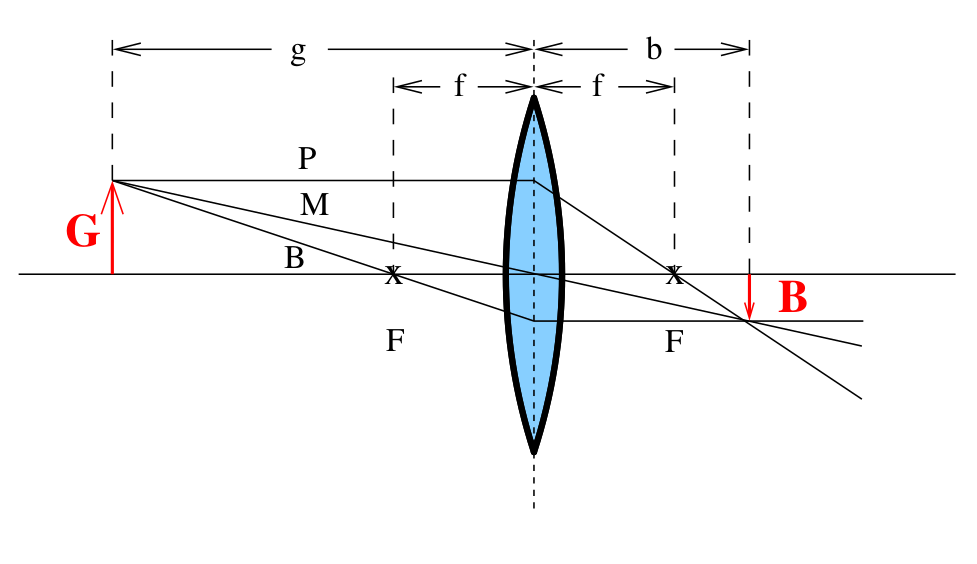
\includegraphics[width=\linewidth]{Bilder/sammellinse.png}
  \caption{Schematischer Strahlverlauf bei einer Sammellinse \cite{Anleitung}}
  \label{fig:sammelli}
\end{wrapfigure}
\FloatBarrier
Dieser Effekt wird genutzt, um mittels verschieden geformter Grenzflächen mittels sogenannter Linsen den Strahlverlauf zu verändern.
In der Optik wird zwichen verschiedenen Linsen unterschieden.
Bei dünnen Linsen lässt sich die Brechung auf die Mittelebene der Linse reduzieren.
Eine Sammellinse wird zum Linsenrand hin dünner, sie bündelt parallel einfallendes Licht in dem sogennanten Brennpunkt. Entsprechend sind die Brennweite $f$ und die Bildweite $b$ positiv gezählt und es ensteht, wie in Abbildung \ref{fig:sammelli} dargestellt, ein reeles Bild.
Unter dem Begriff reeles Bild wird ein Bild verstanden, von dem reale Strahlen ausgehen. Im Gegensatz dazu ist ein virtuelles Bild ein Bild von dem keine reale Strahlen ausgehen so suggeriert ein Blick in den Spiegel zum Beispiel, dass sich Objekte ebenso weit hinter dem Spiegel stehen, wie sie im Realen vor dem Spiegel sind.

%Jaaa nice wrapfigures mal wieder!!!11
\begin{wrapfigure}{r}{0.48\textwidth}
  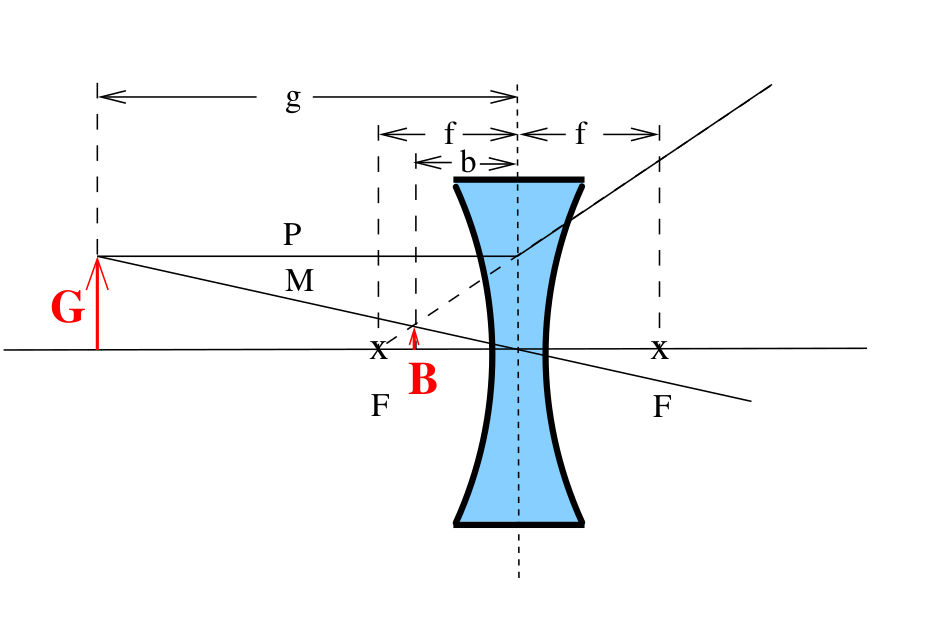
\includegraphics[width=\linewidth]{Bilder/streulinse.png}
  \caption{Schematischer Strahlverlauf bei einer Streulinse \cite{Anleitung}}
  \label{fig:streuli}
\end{wrapfigure}
Ebenso entsteht ein virtuelles Bild bei einer Streulinse (vlg. Abbildung \ref{fig:streuli}).
Die einfallende Strahlen werden nicht fokussiert, sondern vom Zentrum weggebrochen. Die gedachte Verlängerung der Strahlen auf der Gegenstandsseite der Linse führt schließlich zum virtuellen Bild. Daher sind Bildweite und Brennweite auch negativ gezählt.

Im Gegensatz zu dünnen Linsen ist die Reduktion der Brechung nur auf die Mittelebene bei dicken Linsen nicht möglich. Stattdessen werden zwei Hauptebenen eingeführt und die Brechung der einfallenden Strahlen an ihnen, wie in Abbildung \ref{fig:diefette} dargestellt, vorgenommen.
Es wird vereinfachend angenommen, dass zwischen den beiden Hauptebenen der Linse alle Strahlen parallel laufen.

Die Bildkonstruktion bei einer Linse erfolgt über die Ausnutzung der Eigenschaften dreier ausgezeichneter Strahlen. Diese werden im Folgenden anhand der dünnen Sammellinse (Abbildung \ref{fig:sammelli}) beispielhaft erläutert.
Der Parallelstrahl $P$ verläuft ausgehend vom Gegenstandspunkt parallel zur optischen Achse, also der Symmetrieachse des rotationssymmetrischen optischen Systems, wird an der Mittelebene gebrochen, und läuft bildseitig als Brennpunktstrahl durch selbigen zum Bildpunkt.
Der Brennpunktstrahl $B$ läuft gegenstandsseitig durch den Brennpunkt und wird nach der Brechung an der Mittelebene zum Parallelstrahl.
Der Mittelpunktsstrahl $M$ wird gar nicht gebrochen, sondern läuft direkt vom Gegenstandspunkt, durch den Linsenmittelpunkt zum Bildpunkt.

\begin{wrapfigure}{r}{0.48\textwidth}
  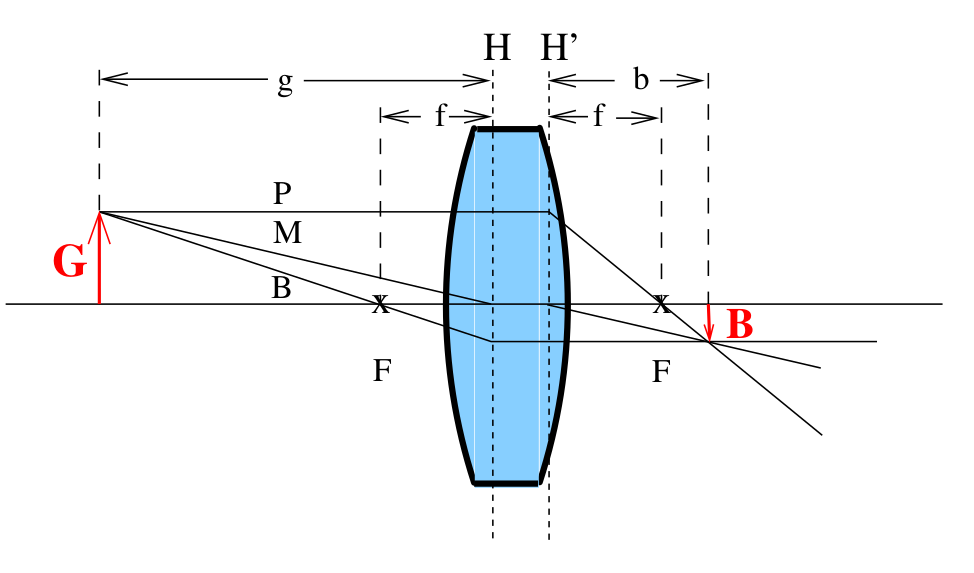
\includegraphics[width=\linewidth]{Bilder/fettelinse.png}
  \caption{Schematischer Strahlverlauf bei einer dicken Sammellinse \cite{Anleitung}}
  \label{fig:diefette}
\end{wrapfigure}
Die Betrachtung der Konstruktionsstrahlen führt unter Verwendung der Strahlensätze auf das Abbildungsgesetz:
\begin{equation}
  \label{eqn:abbi}
  V=\frac{B}{G}=\frac{b}{g} \text{.}
\end{equation}
Der Abbildungsmaßstab $V$ ist also gleich dem Verhältnis aus Bildgröße $B$ und Gegenstandsgröße $G$. Diese verhalten sich zudem zueinander wie die Bildweite $b$ zur Gegenstandsweite $g$.
Unter erneuter Verwendung des Strahlensatzes ergibt sich aus der Bildkonstruktion der dünnen Linse die Linsengleichung
\begin{equation}
  \label{eqn:linsi}
\frac{1}{f}=\frac{1}{b}+\frac{1}{g} \text{.}
\end{equation}
Die Linsengleichung behält auch ihre Gültigkeit für dicke Linsen, allerdings müssen die Brennweite $f$, sowie Gegenstands-und Bildweite bezüglich der Hauptebenen einzeln bestimmt werden.
Die verwendete Reduktion der Brechung gilt strenggenommen nur für Strahlen nahe der optischen Achse. Für achsenferne Strahlen treten Abbildungsfehler auf.
Bei der sphärischen Abberration werden achsenferne Strahlen stärker gebrochen als achsennahe strahlen, sodass ihr Brennpunkt nicht mehr zusammenfällt und infolgedessen ein unscharfes Bild entsteht.
Bei der chromatischen Abberration wird aufgrund der Dispersion das Licht in seine Spektralfarben zerlegt. Somit liegt der Brennpunkt des kurzwelligen Lichts (blau) näher an der Linse als der des langwelligen, roten Lichts.

Die Brechkraft $D$ wird definiert als reziproke Brennweite $D=\frac{1}{f}$. Die Brechkraft eines Linsensystems ergibt sich wiederum aus der der Summe der Brechkräfte $D_{\mathrm{i}}$ der einzelnen Linsen des Systems.
\FloatBarrier
\subsection{Methode von Bessel zur Bestimmung der Brennweite $f$ einer Linse}
Zur Bestimmung der Brennweite wird der Abstand $e$ zwischen Gegenstand und Bild festgehalten und die beiden Linsenpositionen gesucht, bei denen das Bild scharf abgebildet wird.
Diese Linsenanordnung ist symmetrisch, es werden Bildweite und Gegenstandsweite vertauscht.
Es ergeben sich somit die Relationen
\begin{equation}
b_{\mathrm{1}}=g_{\mathrm{2}} \text{und} b_{\mathrm{2}}=g_{\mathrm{1}} \text{.}
\end{equation}
Über den Abstand $e=b_{\mathrm{1}}+g_{\mathrm{}}=b_{\mathrm{2}}+g_{\mathrm{2}} $ zwischen Gegenstand und Bild, sowie der Distanz $d=g_{\mathrm{1}}-b_{\mathrm{1}}=g_{\mathrm{2}}-b_{\mathrm{2}}$ zwischen den beiden Linsenpositionen an denen ein scharfes Bild auf dem Schirm entsteht,
ergibt sich die Brennweite der Linse zu
\begin{equation}
  f=\frac{e^2-d^2}{4e}\text{.}
\end{equation}

\subsection{Methode von Abbe zur Bestimmung der Brennweite eines Linsensystems}
Bei der Methode von Abbe werden die Bildweite $b$ und die Gegenstandsweite $g$ eines Linsensystems bezüglich seiner Hauptebenen gemessen. Deren Position ist nicht bekannt, daher wird bezüglich eines beliebigen Referenzpunktes $A$ die Gegenstandsweite $g'$ und die Bildweite $b'$ gemessen.
Zudem wird der Abbildungsmaßstab $V$ benötigt.
Für die Hilfsgrößen gilt (vgl. Abbildung \ref{fig:abbe}):
\begin{gather}
  \label{eqn:abbe}
  g'=g+h=f\cdot\left(1+\frac{1}{V}\right)+h \text{,}\\
  b'=b+h'=f\cdot\left(1+V\right)+h' \text{.}\\
\end{gather}
Die Lage der Hauptebenen $H$ und $H'$, sowie die Brennweite $f$ des Linsensystems lassen sich nun berechnen.
